\chapter{Interfaz}
\label{cap:interfaz}

Uno de los principales objetivos del presente trabajo era aunar todas las funcionalidades de la aplicación original, así como las extensiones implementadas en este desarrollo, en una única interfaz web, mediante la cual el usuario pueda navegar y acceder a todas las funcionalidades disponibles.

En cuanto a la movilidad entre páginas, se ha implementado una barra de navegación, la cual compartirán todas las páginas y permitirá navegar entre las diferentes funcionalidades, como se puede apreciar en las figuras \ref{fig:navBarDesktop} y \ref{fig:navBarMobile}.

\begin{figure}[h]
	\centering
	
\includegraphics[width = 1\textwidth]{Imagenes/Vectorial/navBarDesktop.png}
	\caption{Barra de navegación en el formato Desktop}
	\label{fig:navBarDesktop}
\end{figure}

\begin{figure}[h]
	\centering
	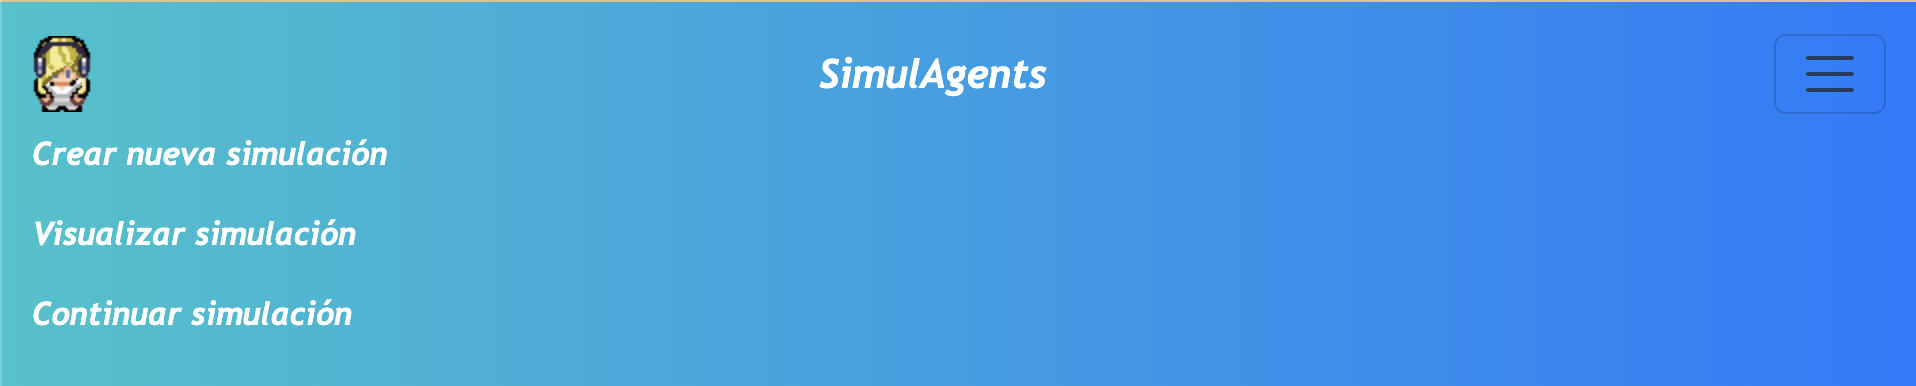
\includegraphics[width = 1\textwidth]{Imagenes/Vectorial/navBarMobile.png}
	\caption{Barra de navegación en el formato para dispositivos móviles}
	\label{fig:navBarMobile}
\end{figure}

\section{Vista de Crear nueva simulación}

Teniendo en cuenta los objetivos y las funcionalidades implementadas en este trabajo, es evidente la necesidad de un apartado en el que permitir a los usuarios crear sus propias simulaciones. En esta vista, los usuarios primeramente indicarán el número de personajes que quieren que intervengan en la simulación.

Dependiendo del número de personajes deseados, mediante el uso de la tecnología JQuery, se mostrarán u ocultarán las casillas de relleno de la información de los personajes. Para cada uno de los agentes, los usuarios indicarán el nombre que le quieren dar y la personalidad de los mismos. En el apartado de personalidad ,se indican todas sus relaciones sociales preexistentes en lenguaje natural, así como los pensamientos y pretensiones que el agente tiene al inicio de la simulación.

Por último, hay un apartado de contexto de la simulación, en el cual los usuarión deberán insertar todo el contexto de la situación en la que se ejecute la simulación. En esta información entraría el día en el que se ejecuta, la situación en la que se encuentran los personajes y todo tipo de información que pueda aportar contexto a la simulación.

Todas estos elementos gráficos se pueden apreciar en la figura \ref{fig:vistaCrearSimulacion}.

\begin{figure}[h]
	\centering
	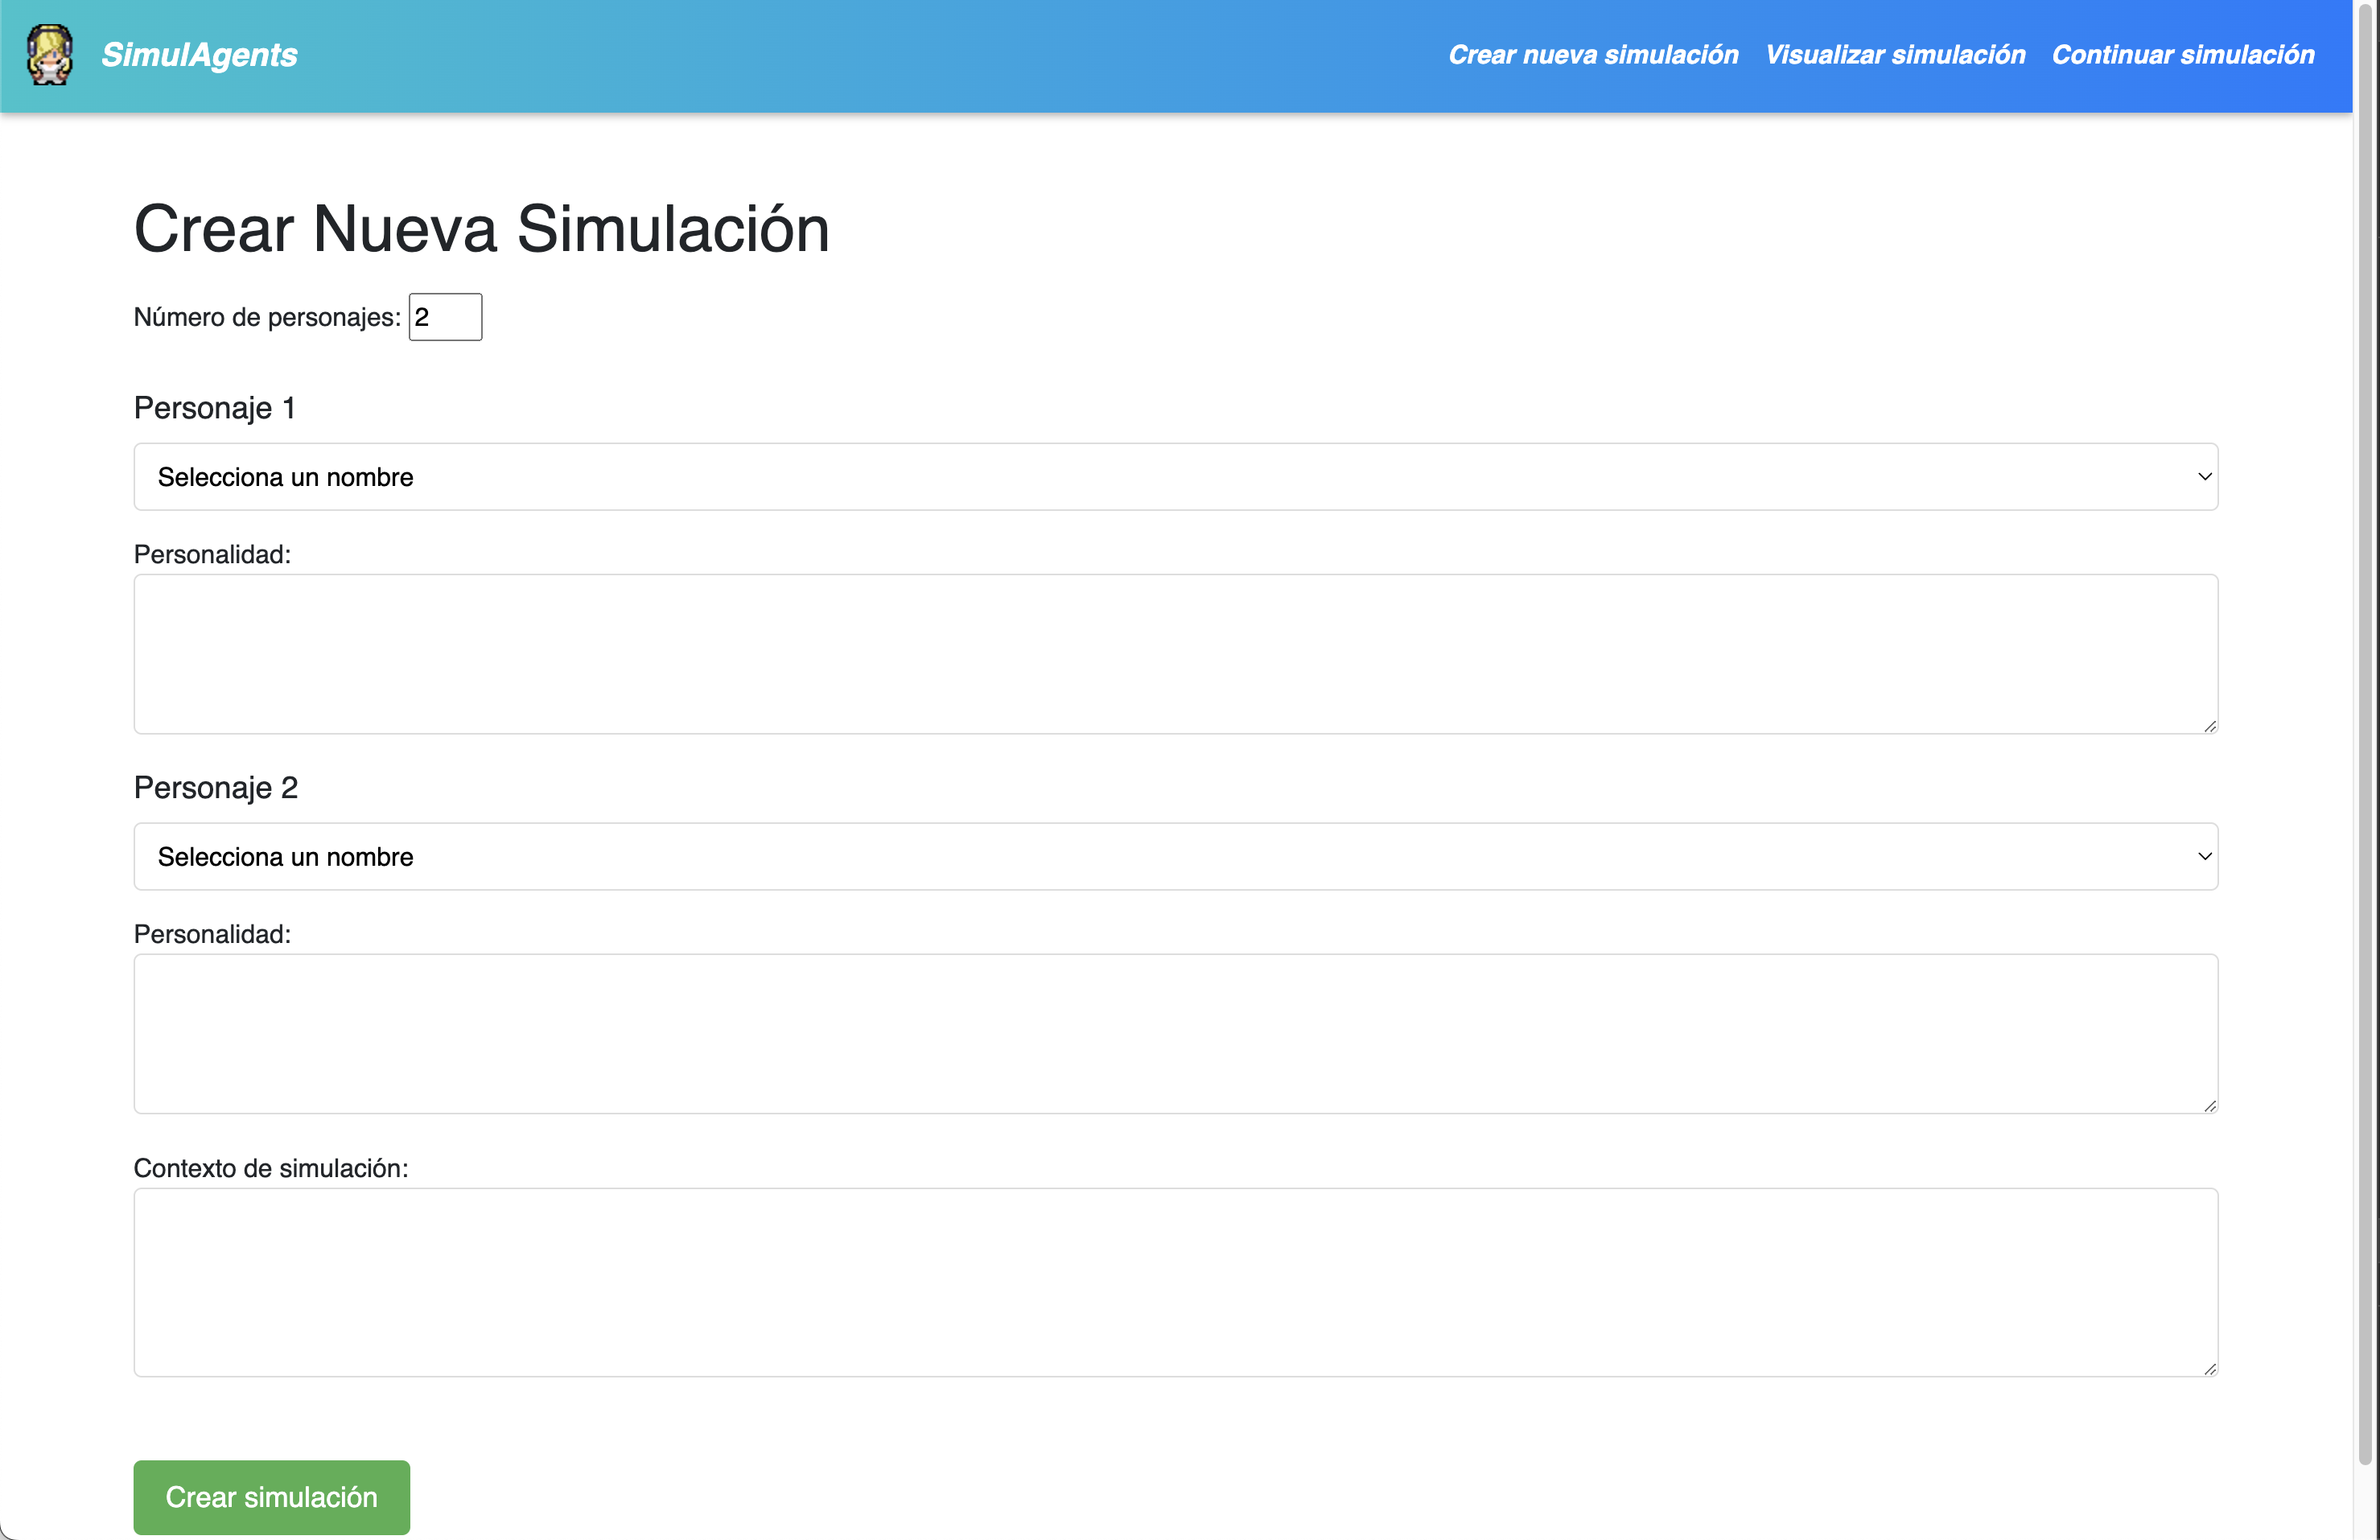
\includegraphics[width = 1\textwidth]{Imagenes/Vectorial/vistaCrearSimulacion.png}
	\caption{Versión de escritorio de la vista para crear una nueva simulación}
	\label{fig:vistaCrearSimulacion}
\end{figure}

\section{Vista de Visualizar simulación}

\section{Vista de Continuar simulación}

\section{Vista de Guía de Usuario}
